\documentclass[8pt]{beamer}\usepackage[]{graphicx}\usepackage[]{color}

\usetheme{metropolis}           % Use metropolis theme
\usepackage{amsmath}
\usepackage{mathrsfs}
\usepackage{tabularx}
\usepackage{tikz}
\usetikzlibrary{patterns}

% For custom oversets
\usepackage{accents}

% For addmargin
\usepackage{scrextend}


\usepackage[style=authoryear]{biblatex}
\addbibresource{references.bib}
\usepackage{cleveref}
\renewcommand*{\bibfont}{\footnotesize}


\def\coingrid{
\draw[step=1cm,gray,very thin] (0,0) grid (2,3);
\node[left, color=blue] at (0, 2.5) {Coin TT};
\node[left, color=blue] at (0, 1.5) {Coin HT};
\node[left, color=blue] at (0, 0.5) {Coin HH};
\node[above, color=purple] at (0.5, 3) {Side 1};
\node[above, color=purple] at (1.5, 3) {Side 2};
\node[below right, color=black] at (0, 3) {\tiny TT1};
\node[below right, color=black] at (0, 2) {\tiny HT1};
\node[below right, color=black] at (0, 1) {\tiny HH1};
\node[below right, color=black] at (1, 3) {\tiny TT2};
\node[below right, color=black] at (1, 2) {\tiny HT2};
\node[below right, color=black] at (1, 1) {\tiny HH2};
}

\def\rectfill#1#2#3#4{
\draw[pattern=#1, pattern color=#2] (#3,#4) rectangle (#3 + 1,#4 + 1);
}


\def\truth{${\color{red}\times}$}

\def\heads{
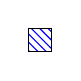
\begin{tikzpicture}[scale=0.30]
    \rectfill{north west lines}{blue}{0}{1}
\end{tikzpicture}
}

\def\ttcoin{

\begin{tikzpicture}[scale=0.30]
    \draw[draw=lime, thick] (0, 1) rectangle ++(1, 1);
\end{tikzpicture}
}

\def\htcoin{

\begin{tikzpicture}[scale=0.30]
    \draw[draw=red, thick] (0, 1) rectangle ++(1, 1);
\end{tikzpicture}
}

\def\hhcoin{

\begin{tikzpicture}[scale=0.30]
    \draw[draw=cyan, thick] (0, 1) rectangle ++(1, 1);
\end{tikzpicture}
}


\def\hiprop{

\begin{tikzpicture}[scale=0.30]
    \rectfill{north east lines}{red}{0}{1}
\end{tikzpicture}
}



\def\setminipage{

\begin{minipage}{0.38\textwidth}
    \begin{center}
    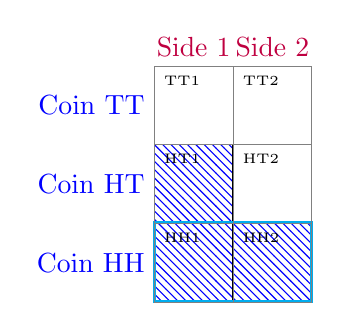
\begin{tikzpicture}
        \rectfill{north west lines}{blue}{0}{0}
        \rectfill{north west lines}{blue}{0}{1}
        \rectfill{north west lines}{blue}{1}{0}
        % \draw[draw=red, very thick] (0, 1) rectangle ++(2, 1);
        % \draw[draw=lime, very thick] (0, 2.01) rectangle ++(2, 1);
        \draw[draw=cyan, very thick] (0, 0.01) rectangle ++(2, 1);
        \coingrid{}
    \end{tikzpicture}
\end{center}
\end{minipage}
\begin{minipage}{0.58\textwidth}
    %
    \heads{} We observe heads = $HT1 \lor HH1 \lor HH2$

    % \ttcoin{} We chose the TT coin = $TT1 \lor TT2$

    % \htcoin{} We chose the HT coin = $HT1 \lor HT2$

    \hhcoin{} We chose the HH coin = $HH1 \lor HH2$

    Recall that the truth \truth{} lies in exactly one cell.

\end{minipage}

}


\def\pmminipage{

\begin{minipage}{0.38\textwidth}
    \begin{center}
    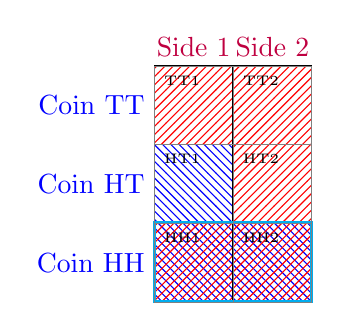
\begin{tikzpicture}
        \rectfill{north west lines}{blue}{0}{0}
        \rectfill{north west lines}{blue}{0}{1}
        \rectfill{north west lines}{blue}{1}{0}
        \rectfill{north east lines}{red}{0}{0}
        \rectfill{north east lines}{red}{1}{0}
        \rectfill{north east lines}{red}{1}{1}
        \rectfill{north east lines}{red}{1}{2}
        \rectfill{north east lines}{red}{0}{2}

        \draw[draw=cyan, very thick] (0, 0.01) rectangle ++(2, 1);
        \coingrid{}
    \end{tikzpicture}
\end{center}
\end{minipage}
\begin{minipage}{0.58\textwidth}
    %
    \heads{} $e$ = We observe heads\\
    \hhcoin{} $h$  = We chose the HH coin\\
    \heads{} $h_D$ = Inductive component = $h \lor e = e$\\
    \hiprop{} $h_I$ = Inductive component = $h \lor \lnot e$

    \vspace{1em}
    We can write $h = h_D \land h_I$.\\

    Note also that $h \subseteq e$ so $h_D = e$.
    %
\end{minipage}

}


\def\p#1{\mathbb{P}\left(#1\right)}
\def\q#1{\mathbb{Q}\left(#1\right)}
\def\y{y}
\def\z{z}
\def\normz{\mathcal{N}(z)}
\def\etahat{\hat{\eta}}
\def\ellhat{\hat{\ell}}
\def\sumn{\sum_{n=1}^N}
\def\meann{\frac{1}{N} \sumn}
\newcommand{\etastar}{\accentset{*}{\eta}}
\def\Z{\mathcal{Z}}
\def\expect#1#2{\mathbb{E}_{#1}\left[#2\right]}
\def\kl#1{\mathrm{KL}\left(#1\right)}
\def\klhat#1{\widehat{\mathrm{KL}}\left(#1\right)}
\def\ind#1{1\left(#1\right)}

\DeclareMathOperator*{\argmax}{\mathrm{argmax}}
\DeclareMathOperator*{\argmin}{\mathrm{argmin}}
\DeclareMathOperator*{\esssup}{\mathrm{esssup}}
\DeclareMathOperator*{\essinf}{\mathrm{essinf}}
\DeclareMathOperator*{\argsup}{\mathrm{argsup}}
\DeclareMathOperator*{\arginf}{\mathrm{arginf}}

\title{Inductive logic: Introduction and context}
\author{Ryan Giordano}
\date{Sep 23rd, 2022}
\institute{Massachusetts Institute of Technology}

\begin{document}


%%%%%%%%%%%%%%%%%%%%%%%%%%%%%%%%%%%%%%%%%%%%%%%%%%%%%%%%%%%%%%%%%%%%%%%
%%%%%%%%%%%%%%%%%%%%%%%%%%%%%%%%%%%%%%%%%%%%%%%%%%%%%%%%%%%%%%%%%%%%%%%
%%%%%%%%%%%%%%%%%%%%%%%%%%%%%%%%%%%%%%%%%%%%%%%%%%%%%%%%%%%%%%%%%%%%%%%

\begin{frame}{Inductive Logic review}

Recall Hume: We have observed the sun rise every day our whole lives.  How are
we justified in believing it will rise again tomorrow?

Hume (and many other logicians) proposes a dichotomy between
%
\begin{itemize}
%
\item Deduction
%
\begin{itemize}
%
\item Certain
\item Mathematical
\item Conclusions contain no more information than the premises
%
\end{itemize}
%
\item Induction
\begin{itemize}
%
\item Uncertain
\item Conjectural
\item Conclusions contain amplify or add to the premises
%
\end{itemize}
%
\end{itemize}
%
\pause
At least two factions emerge in response to Hume:
%
\begin{itemize}
%
\item Falsificationists (e.g. \cite{popper:1963:scienceasfalsification}):
    We do not need inductive logic
%
\item Bayesians (e.g. \cite{carnap:1966:aimofinductivelogic}):
    Bayesian probability formalizes inductive logic
%
\end{itemize}
%
Today I will describe a fascinating skirmish in the war between the
falsificationsists and Bayesians: the Popper-Miller theorem.
%
\end{frame}

%%%%%%%%%%%%%%%%%%%%%%%%%%%%%%%%%%%%%%%%%%%%%%%%%%%%%%%%%%%%%%%%%%%%%%%
%%%%%%%%%%%%%%%%%%%%%%%%%%%%%%%%%%%%%%%%%%%%%%%%%%%%%%%%%%%%%%%%%%%%%%%
%%%%%%%%%%%%%%%%%%%%%%%%%%%%%%%%%%%%%%%%%%%%%%%%%%%%%%%%%%%%%%%%%%%%%%%

\begin{frame}{Running Example}

    \setminipage{}

Here is a running example for this presentation. Suppose a bag contains three
coins: one regular coin (HT), one with both faces tails (TT), and one with both
faces heads (HH).  The coin is flipped, and either the first or second side
comes up.

Exactly one possible outcome
of coin $\times$ side occurs; call this the ``truth.''

\pause
%
Recall logical notation:
%
\begin{itemize}
%
\item $\lor$: Disjunction (logical or)
\item $\land$: Conjunction (logical and)
\item $\lnot$: Negation (logical not)
%
\end{itemize}
%


\end{frame}


%%%%%%%%%%%%%%%%%%%%%%%%%%%%%%%%%%%%%%%%%%%%%%%%%%%%%%%%%%%%%%%%%%%%%%%
%%%%%%%%%%%%%%%%%%%%%%%%%%%%%%%%%%%%%%%%%%%%%%%%%%%%%%%%%%%%%%%%%%%%%%%
%%%%%%%%%%%%%%%%%%%%%%%%%%%%%%%%%%%%%%%%%%%%%%%%%%%%%%%%%%%%%%%%%%%%%%%

\begin{frame}{Running Example}

\setminipage{}

Let us define a ``hypothesis'' $h$ and evidence $e$:
%
\begin{itemize}
%
\item Hypothesis $h$: We selected the HH coin (all future flips will be H)
\item Evidence $e$: We observed heads.
%
\end{itemize}
%
How much does $e$ support $h$?  This is an inductive question!  Call the answer
$s(h | e)$.

\pause
Bayes' rule gives a potential answer:
%
\begin{align*}
%
s(h | e) = p(h | e) - p(h).
%
\end{align*}
%
In this case,
%
\begin{align*}
%
s(h | e) = \frac{2}{3} - \frac{1}{3}  = \frac{1}{3} > 0.
%
\end{align*}
%
This is positive, so we might say that $e$ supports $h$.
Have we solved induction?
%
\end{frame}


%%%%%%%%%%%%%%%%%%%%%%%%%%%%%%%%%%%%%%%%%%%%%%%%%%%%%%%%%%%%%%%%%%%%%%%
%%%%%%%%%%%%%%%%%%%%%%%%%%%%%%%%%%%%%%%%%%%%%%%%%%%%%%%%%%%%%%%%%%%%%%%
%%%%%%%%%%%%%%%%%%%%%%%%%%%%%%%%%%%%%%%%%%%%%%%%%%%%%%%%%%%%%%%%%%%%%%%

\begin{frame}{The Popper-Miller theorem}

\setminipage{}

% \pmminipage{}

Popper and Miller say no (\cite{popper:1983:impossibilityinductiveprobability}).

The first step of their argument is to break $h$ into deductive and inductive
components.

\pause
%
\begin{enumerate}
%
\item $e$ follows deductively from $h$, since $h \subseteq e$.
\item But $h$ does not follow deductively from $e$, because $e \nsubseteq h$.
\item Does some ``component'' of $h$ follow from $e$?
\item The strongest proposition implied by $e$ and containing
   $h$ is $h_D := h \lor e$.
\item Can we write $h = h_D \land S$ for some set?
\item The weakest such propostion is $h_I := h \lor \lnot e$.
%
\end{enumerate}
%
So we can write $h = h_D \land h_I$.  Popper and Miller call:
%
\begin{itemize}
%
\item $h_D:$ The ``deductive'' component of $h$
\item $h_I:$ The ``inductive'' component of $h$
%
\end{itemize}
%
\end{frame}


%%%%%%%%%%%%%%%%%%%%%%%%%%%%%%%%%%%%%%%%%%%%%%%%%%%%%%%%%%%%%%%%%%%%%%%
%%%%%%%%%%%%%%%%%%%%%%%%%%%%%%%%%%%%%%%%%%%%%%%%%%%%%%%%%%%%%%%%%%%%%%%
%%%%%%%%%%%%%%%%%%%%%%%%%%%%%%%%%%%%%%%%%%%%%%%%%%%%%%%%%%%%%%%%%%%%%%%

\begin{frame}{The Popper-Miller theorem}

\pmminipage{}

What is the support for these two components?  Basic calculations show that
%
\begin{align*}
%
s(h_D | e)
    ={}&& p(h_D | e) - p(h_D)
    % ={}&& p(h \lor e | e) - p(h \lor e)
    ={}&& 1 - p(e) \\
s(h_I | e)
    ={}&& p(h_I | e) - p(h_I)
    % ={}&& p(h \lor \lnot e | e) - p(h \lor \lnot e)
    ={}&& p(h | e) - (p(h) + 1 - p(e))\\
%
\Rightarrow
s(h | e)
    ={}&& p(h | e) - p(h)
    ={}&&
    s(h_D | e) + s(h_I | e)
\end{align*}
%
So the support of $h$ is the sum of the support for its
components.  \pause Next, by Bayes' rule,
%
\begin{align*}
%
s(h | e)
    ={} \frac{p(h \land e)}{p(e)} - p(h)
    ={} \frac{p(h)}{p(e)} - p(h)
    ={} \frac{p(h)}{p(e)}\left(1 - p(e) \right)
    <{} 1 - p(e)
    ={} s(h_D | e).
%
\end{align*}
%
So $h$ is supported less than its deterministic component.  Also sensible.
\pause
But then:
%
\begin{align*}
%
s(h_I | e) = s(h | e) - s(h_D | e) < 0.
%
\end{align*}
%
\textbf{$\Rightarrow$ The inductive component is counter-supported by the evidence.}
%
\end{frame}


%%%%%%%%%%%%%%%%%%%%%%%%%%%%%%%%%%%%%%%%%%%%%%%%%%%%%%%%%%%%%%%%%%%%%%%
%%%%%%%%%%%%%%%%%%%%%%%%%%%%%%%%%%%%%%%%%%%%%%%%%%%%%%%%%%%%%%%%%%%%%%%
%%%%%%%%%%%%%%%%%%%%%%%%%%%%%%%%%%%%%%%%%%%%%%%%%%%%%%%%%%%%%%%%%%%%%%%

\begin{frame}{The Popper-Miller theorem}
%
To summarize Popper-Miller's argument:
%
\begin{enumerate}
%
\item We can write $h = h_D \land h_I$ where $h_D$ follows deductively from $e$.
\item We have chosen $h_I$ so that $s(h | e) = s(h_D | e) + s(h_I | e)$.
\item It is reasonable to call $h_D$ and $h_I$ the deductive and
inductive components of $h$.
\item But $s(h_D | e) > s(h | e)$, so $s(h_I | e) < 0$.
%
\end{enumerate}
%
That is, $h$ is only supported by $e$ because
it depends partly, deductively, on $e$.

Any non-deductive dependence of $h$ on $e$ is actually
{\em counter-supported} by the evidence.

\textbf{The fact that we appear to be doing induction is a mirage.}

\pause

\begin{addmargin}[2em]{2em}% 1em left, 2em right
``This result is completely
devastating to the inductive interpretation of the calculus of probability. All
probabilistic support is purely deductive: that part of a hypothesis that is not
deductively entailed by the evidence is always strongly countersupported by
the evidence --- the more strongly the more the evidence asserts.''\\
(\cite{popper:1983:impossibilityinductiveprobability})
\end{addmargin}

\end{frame}

%%%%%%%%%%%%%%%%%%%%%%%%%%%%%%%%%%%%%%%%%%%%%%%%%%%%%%%%%%%%%%%%%%%%%%%
%%%%%%%%%%%%%%%%%%%%%%%%%%%%%%%%%%%%%%%%%%%%%%%%%%%%%%%%%%%%%%%%%%%%%%%
%%%%%%%%%%%%%%%%%%%%%%%%%%%%%%%%%%%%%%%%%%%%%%%%%%%%%%%%%%%%%%%%%%%%%%%
\begin{frame}{The discussion continues}
%
This idea generated a lot of discussion, and a detailed
follow-up by Popper and Miller.  Some notable references:
%
\begin{itemize}
%
\item \cite{levi:1984:impossibility}
\item \cite{redhead:1985:impossibility}
\item \cite{levi:1986:probabilisticpettifoggery}
\item \cite{good:1990:suspiciouspoppermiller}
\item \cite{popper:1987:probabilistic}
%
\end{itemize}
%
To me, this result has the feel of a paradox.  Though maybe not very practically
relevant, by taking it seriously one is forced to think very carefully and
potentially identify unarticulated assumptions or unjustified conculsions.

\textbf{What do you think?}

\end{frame}

%%%%%%%%%%%%%%%%%%%%%%%%%%%%%%%%%%%%%%%%%%%%%%%%%%%%%%%%%%%%%%%%%%%%%%%
%%%%%%%%%%%%%%%%%%%%%%%%%%%%%%%%%%%%%%%%%%%%%%%%%%%%%%%%%%%%%%%%%%%%%%%
%%%%%%%%%%%%%%%%%%%%%%%%%%%%%%%%%%%%%%%%%%%%%%%%%%%%%%%%%%%%%%%%%%%%%%%

\begin{frame}{Bibliography}
\printbibliography{}
\end{frame}

\end{document}
